% TEMPLATE for Usenix papers, specifically to meet requirements of
%  USENIX '05
% originally a template for producing IEEE-format articles using LaTeX.
%   written by Matthew Ward, CS Department, Worcester Polytechnic Institute.
% adapted by David Beazley for his excellent SWIG paper in Proceedings,
%   Tcl 96
% turned into a smartass generic template by De Clarke, with thanks to
%   both the above pioneers
% use at your own risk.  Complaints to /dev/null.
% make it two column with no page numbering, default is 10 point

% Munged by Fred Douglis <douglis@research.att.com> 10/97 to separate
% the .sty file from the LaTeX source template, so that people can
% more easily include the .sty file into an existing document.  Also
% changed to more closely follow the style guidelines as represented
% by the Word sample file. 

% Note that since 2010, USENIX does not require endnotes. If you want
% foot of page notes, don't include the endnotes package in the 
% usepackage command, below.

% This version uses the latex2e styles, not the very ancient 2.09 stuff.
\documentclass[letterpaper,twocolumn,10pt]{article}
\usepackage{usenix,epsfig,url}
\begin{document}

%don't want date printed
\date{}

%make title bold and 14 pt font (Latex default is non-bold, 16 pt)
\title{\Large \bf Webcam Fuzz Testing: Testing IoT Deployments}

%for single author (just remove % characters)
\author{
{\rm Matthew Elbert}\\
University of Utah
\and
{\rm Jeffrey Kitchen}\\
University of Utah
% copy the following lines to add more authors
% \and
% {\rm Name}\\
%Name Institution
} % end author

\maketitle

% Use the following at camera-ready time to suppress page numbers.
% Comment it out when you first submit the paper for review.
\thispagestyle{empty}


\subsection*{Abstract}

With the growing proliferation of Internet of Things (IoT) devices, they could become a very attractive target for malicious attacks. Attacks on these devices, especially ones used for surveillance, would also greatly compromise security. A commerically available example of this is a wireless IP camera.
Fuzz testing, or fuzzing, is a simple, automated method to find bugs and vulnerabilities in programs, where random, potentially invalid inputs are sent. Fuzz testing can be much cheaper than other types of testing and often reveals bugs developers and testers cannot foresee. We use fuzzing methods on two different types of Wi-Fi cameras in order to evaluate the quality of fuzz testing on these recent types of IoT deployments. We used a fuzzing tool called Pathoc within a Bash shell script framework for crafted malice towards the HTTP servers in these cameras, and ran over 250,000 fuzzing tests. We did identify several interesting events and responses from fuzzing tests, but did not identify any critical bugs or serious vulnerabilities in the cameras. 



The specific `call for papers' that we target in the presentation of this research is the 9th USENIX Workshop on Offensive Technologies (WOOT '15). \url{https://www.usenix.org/conference/woot15/call-for-papers}

\section{Introduction}

Fuzz testing is a method of testing in which random, potentially invalid inputs are sent to a program or service in order to test for vulnerabilities. It is often used as either a gray or black-box testing platform for security testing. Fuzz testing can be a very cheap and effective implementation of testing as many inputs can be generated, sent, and analyzed automatically, without the need for a human to monitor. However, a truly random test input could easily not provide anything useful in a reasonable amount of time. Therefore, many solutions (citations needed) propose a different method where random mutation of good inputs is used so that requests that are close to being correct are used. 
Because the world has become more internet-connected than ever, fuzz testing can be an important tool for developers as network-facing interfaces can experience any input, and need to be tested for this randomness. However, many functions are very state-driven, and a true, random test may only test a single interface, and not the whole system. Because of this, many of these fuzz testers must be stateful in order to do a complete test. Because of many security issues with the current Internet architecture, there are obviously some security measures put in place to almost anything that is deployed on a network, even if it is meant to only be local. Therefore, something as simple as logging into an interface needs to be taken into account in order to get more meaningful tests.

After an initial period of exploring current research in fuzzing, we settled on this goal: \textit{Can we use fuzzing to discover interesting bugs or vulnerabilities in a network-connected device?} Reaching this goal involved several steps: choosing a service to test; deciding how to generate random inputs; determining how to distinguish "good" and "bad" test results; implementing the random tester; and evaluating the effectiveness of the test procedure. 

Initially, we set out to design our own fuzzer, but in researching the subject showed that may tools were already available, which allowed us to focus on trying to find undiscovered bugs and vulnerabilities, instead of the effectiveness of an implementation. A very basic and highly proliferated technology deployed on the internet is an HTTP server. But because of this prevalence, popular servers such as Apache have been thoroughly tested and documented. However, more and more devices are being connected, with an uptake in the Internet of Things (IoT) mentality. Therefore, we chose wireless IP cameras as the platform to fuzz test. These are some of the most widely available IoT devices for consumers, and could become an attractive entry point for attackers. We found that the two devices we purchased ran basic HTTP servers, and we could use tools made for these applications. If these devices could be accessed by unauthorized third parties, or be made unable to perform their duties, this could be a serious issue. We believe that fuzz testing can be an effective way to study if these bugs or vulnerabilities exist. 


\section{Related Work} 

One of the first attempts at a random input tester was done by Miller et. al.~\cite{millerUNIX}. Their work consisted of creating small programs for UNIX that would generate random strings that would then be piped to various programs of a few UNIX distributions. They found, at the time of publication in 1990, that they could cause roughly a third of the tested utilities to crash or hang with the generated inputs, some of which even caused UNIX crashes.

SNOOZE~\cite{snooze} is a network fuzzing protocol that is used to test the security of network protocols. In their approach, they show how the true random testing of fuzzing would not be desirable for the protocols in which they wanted to test. Therefore, they created a method in which the state machines of protocols are defined, and then transversed through the testing. SNOOZE chose to focus on the Session Initiation Protocol (SIP), which is a key protocol for VoIP calls.

SecFuzz~\cite{secfuzz} was another implementation of testing security protocols. For their tests, they focused on the Internet Key Exchange (IKE) protocols, and gave their fuzzer the necessary cryptographic functions. Their method entailed sending correct inputs in order to get the state-driven protocol into a desired state, and then slowly mutate good inputs for that state until something undesirable happened. They relied on what they called ``fuzz operators" that would set certain fields, payloads or messages to certain values (eg. random or zero) to try and coax an undesirable response.

AspFuzz~\cite{aspfuzz} was another type of fuzzer, but this one was created and tested in protocols such as POP and HTTP. Their implementation had a user supply the protocol specification. It would then generate attacks that would either be long strings, known incorrect characters, known out of bounds numbers, format strings, changing the number of fields, and removing delimiters. 

While these papers looked like they had gathered results from their fuzz testing, they did not release their prototype to the public, and therefore we had to find other publicly available tools that would be able to create fuzz tests. A few of the papers read, such as AspFuzz, mentioned the Peach Fuzzing Platform~\cite{peach} as a tool widely used in this type of testing. We were also able to find widely available tools like AutoFuzz~\cite{autofuzz}, American Fuzzy Lop (AFL)~\cite{afl}, and Pathod/Pathoc~\cite{pathod}. More discussion on these tools is presented in section 3.1.2.

We tried to find research related to fuzzing internet-connected devices, but were unable to. Therefore, we thought this might be a good starting point for our research. We thought this would be important because more and more `things' are connecting to the internet today, and all of these `Internet of Things' devices have network protocols that would be interesting to test. 

\section{Experimental Methodology}
In order to create meaningful experiments, the devices under test had to be purchased and evaluated further. Points of attack had to be gathered, evaluated, and implemented in the available tools in order to better attempt to find interesting results.   

\subsection{IP Cameras}
The two cameras we purchased were a D-Link Day \& Night Wi-Fi Camera (DCS-934L)~\cite{dlinkCam} and a Pyle Home Indoor Wireless/Wired P2P IP Network Camera (PIPCAM5). The cameras support the following protocols:
\begin{itemize}
	\itemsep-.5em
	\item IPv4, ARP, TCP, UDP, ICMP
	\item DHCP Client
	\item NTP Client (D-Link only)
	\item DNS Client
	\item DDNS Client
	\item SMTP Client
	\item FTP Client
	\item HTTP Server
	\item PPPoE
	\item UPnP port forwarding
	\item RTP, RTSP, RTCP (D-Link only)
	\item LLTD (D-Link only)
	\item GPRS (Pyle only)
\end{itemize}
Though both cameras supported many network protocols, we focused on fuzzing the \textit{alphapd} and \textit{mini-httpd} HTTP servers and the application layers of each of the cameras. We thought the HTTP server protocols and application layers would be the most interesting to fuzz. Most of the other protocols supported were only client protocols, which we felt would be less interesting to fuzz, yet still valuable. We leave testing these other protocols for future work. 


\subsubsection{Information Gathering}
When we first purchased the cameras, we set them up for normal operation and began playing with the provided tools to learn about how they worked. Each of the cameras, after being set up properly, were assigned IP addresses where their main web pages could be accessed. Access to these web pages is protected by username/password combinations defined during the setup process. Once logged in, a number of functions and features are available. For example, on the D-Link camera, the user can manually select day or night mode, enable or disable motion or sound detection, turn on and off notification emails, etc. The Pyle camera also allowed Panning and Tilting via the network.

While the many supported protocols provided many different access points, it was important to identify how the protocol was being implemented. The majority of services running on the cameras were client protocols, such as sending SMTP mail or an image transfer via FTP. This then gave greater incentive in focusing on the HTTP protocol, as it was the only server. The nature of a server is very appealing to an attack, as it is readily available to accept user inputs, and the biggest ``front door" to the cameras.

The first step we took in identifying points of access that could be `fuzzable' was to capture some traffic from the cameras in Wireshark~\cite{wireshark}. We also looked at the HTML source behind the web pages to discover potential attack points. We discovered early on that authentication tokens could be easily exposed, making deeper application level access possible. This was possible because the cameras only used Basic or Digest Authentication, where the encoded user name and password are stored in plain text in the requests. From here, we could automate the fuzzer to get past the HTTP ``front door" and send sensitive commands that require authentication. This way, we could also test the application layer being run on these camera, rather than the HTTP protocol layer. We discovered several `.cgi' pages under the main HTML pages that were the primary interfaces to the camera functions, and we used these pages to fuzz application layers.

We found the following cgi pages for the DLINK camera: 


\begin{enumerate}
	\item /audiocontrol.cgi - METHOD=``POST" name=``AudioMute" value=``[0$\mid$1]"
	\item /nightmodecontrol.cgi - METHOD=``POST" name=``IRLed" value=``[0$\mid$1]"
	\item /image/jpeg.cgi
\end{enumerate}

We found the following cgi pages for the Pyle camera:
\begin{enumerate}
	\item /decoder\_control.cgi?command=[0$\mid$100]
	\newline Valid command numbers:
	\begin{verbatim}
	var R320_240=8;
	var R640_480=32;
	var ptz_type=0;	
	var PTZ_STOP=1;
	var TILT_UP=0;
	var TILT_UP_STOP=1;
	var TILT_DOWN=2;
	var TILT_DOWN_STOP=3;
	var PAN_LEFT=4;
	var PAN_LEFT_STOP=5;
	var PAN_RIGHT=6;
	var PAN_RIGHT_STOP=7;
	var PTZ_LEFT_UP=90;
	var PTZ_RIGHT_UP=91;
	var PTZ_LEFT_DOWN=92;
	var PTZ_RIGHT_DOWN=93;
	var PTZ_CENTER=25;
	var PTZ_VPATROL=26;
	var PTZ_VPATROL_STOP=27;
	var PTZ_HPATROL=28;
	var PTZ_HPATROL_STOP=29;
	var PTZ_PELCO_D_HPATROL=20;
	var PTZ_PELCO_D_HPATROL_STOP=21;
	var IO_ON=94;
	var IO_OFF=95;
	\end{verbatim}
	\item camera\_control.cgi?param='+param+'\&value='+value; 
\end{enumerate}

It is important to note that the DLink camera implemented the CGI commands using a HTTP POST method, using the parameters that were passed to it from the application with a command in the body. The Pyle camera, however, took the parameters from the application and then formatted a HTTP GET command, with the CGI commands in the HTTP path, and no body.


\subsubsection{Tools}
We began by exploring a number of available network fuzzers, including Peach, AutoFuzz, American Fuzzy Lop (AFL), and Pathoc. In investigating AFL, we found that it was a tool mainly for file testing, where good files as inputs to tools would be mutated and input back into a program for evaluation. We could have used this to create a file with a valid GET request, ran AFL to mutate, and send the file through something like netcat, but this would be more difficult to control in what gets sent to the servers. This may be a valuable tool for future work in testing the FTP protocols in the cameras.

AutoFuzz has built in support for MSN, SMTP, and FTP protocols, and relied on capturing actual traffic in order to create a state machine. While we did find that both of the cameras used in testing supported both SMTP and FTP, they were only clients, and therefore less likely to accept inputs. We attempted to, but were ultimately not able to capture SMTP or FTP traffic from the cameras. AutoFuzz did not have support for HTTP, so this tool was abandoned.

Peach was another platform that was looked at extensively. The Peach platform relies on ``pits" that define the fields in the standard being tested, as well as the procedure that should be used in testing. Their website shows that they have support for protocols such as HTTP, DHCP, IPv4, IPv6, and IoT protocols like CoAP. However, these pits are how this company makes money, and we were not willing to purchase them in order to evaluate if they would work for us or not.

Pathoc turned out to be fairly simple and straightforward to use, as it was just a command line interface tool that generated HTTP requests such as GET and POST. Because we focused on HTTP, this single protocol application was still very appealing to us. This program allowed us to specify the type of HTTP command, and inject whatever we wanted into the header and body fields while still creating a command with valid syntax. It also has fuzzing capabilities as it is able to inject random bytes anywhere in the request, as well as generate random strings of a desired length and place them in portions of a request. Because of its ease of use and the capability to be used in a simple Bash script, we chose Pathoc v0.14 as our fuzzing platform.


\section{Implementation}

\subsection{Pathoc}
We used Pathoc for crafted malice towards the mini\_httpd and alphapd servers. Pathoc has a built in function to do many requests at one time, but we found that this method had all of the GET requests on a single TCP connection, and therefore made it more difficult to diagnose in programs such as Wireshark. Therefore, since Pathoc can easily be implemented using the command line interface, a shell script was used as a wrapper that would invoke Pathoc multiple times, giving a new HTTP request everytime. In this way, we could also control fairly easily the commands for Pathoc to run, instead of having a single command run multiple times.



\subsection{Scripts}
We wrote a Bash script that would take the IP address, camera ID (1=PYLE, 2=DLINK), and number of fuzzing tests as arguments. Each camera had its own set of fuzzing commands, to make more use of the details we gathered from each individual camera's web page.

A short example from our script is shown below. We used variables to control the inputs to the pathoc command. For example \textit{\$cmd} might represent an HTTP GET or POST, \textit{\$b1} represents the contents of the HTTP body, and \textit{\$auth} represents the header with authentication credentials. The output is checked, and server responses with \textbf{HTTP/1.1 200} are marked `good' and all others are marked `bad'. 
\begin{verbatim}
for (( i=1; i<=$max; i++ ))
do	
d=$(( ($i*100)/$max ))
r=$(( $RANDOM % 100 + 1 )) #Random [1..100]

pathoc -n 1 -t 5 -e -p -q $ip "$cmd$r$b1$auth"
 | tee -a "log_$NOW".txt | tee last_cmd.txt
 | grep 'HTTP/1.1 200' &> /dev/null

if [ $? == 0 ]; then
good=$(( $good+1 ))
#last_out=$(<last_cmd.txt)
#echo "$last_out" >> "log_$NOW""_good.txt"
else
bad=$(( $bad+1 ))
last_out=$(<last_cmd.txt)
echo "$last_out" >> "log_$NOW""_bad.txt"
fi		
echo -ne "Percent Done: $d  \tGood: $good   
\tBad: $bad \r"
done
\end{verbatim}

It is important to note that if the server doesn't respond with \textbf{HTTP/1.1 200}, it does not necessarily mean that it is bad. This is just the metric we used to try and identify possible interesting responses. Some interesting responses we found are detailed in the Results section. Both cameras were tested with and without authorization credentials, in an effort to identify possible security vulnerabilities. 

Fuzzing directed towards the Pyle camera was focused mainly on the \textit{decoder\_control.cgi} page with various commands. We tried commands with valid numbers, invalid (large or negative) numbers, and random strings of various length. 

Fuzzing directed towards the DLink camera were focused in several different categories, including: valid requests sprinkled with random characters, long (70,000 byte) headers, long (70,000 byte) bodies, long (70,000 byte) HTTP GET requests, and HTTP POST to the \textit{audiocontrol.cgi} and \textit{nightmodecontrol.cgi} pages with valid and invalid command bodies. 

We also wrote a separate script to scour the log files and aggregate the total number of responses in various categories. We used some of this data for the Pyle camera to generate tables~\ref{tab:Pyle_Good_CGI} and ~\ref{tab:Pyle_Rand_CGI}. 


\subsection{Platforms}
The primary vehicle for running Pathoc was a Bash script running on a virtual Linux machine inside Oracle's VM VirtualBox 5.0.10. Two different Windows 10 laptops were used to run the VMs. One computer ran a 32-bit Ubuntu 12.04 VM with 2.0GiB of dedicated RAM. The other computer was using the All-in-one SDN App Development Starter VM, an image based off of 64-bit Ubuntu 14.04, from SDNHub.org.

Because these tests can take a significant amount of time, and these computers are also used for other things, a third platform was used to collect fuzzing data. A Raspberry Pi 2 model B (RPi) was used so that Pathoc could be run for an extended amount of time (e.g. over 24 hours) without the platform needing to be used for something else. The Raspberry Pi was running Raspbian, a derivation of Debian, kernel version 4.1.7. The Pi used a USB 802.11n WiFi adapter to connect to the local network, and the fuzzing script and repository for the log files were placed in a connected 16GB USB flash drive.


\section{Results}
We began our research with this question in mind: \textit{Can we use fuzzing to discover interesting bugs or vulnerabilities in a network-connected device?} At this point in our research, we have not identified any critical bugs in the cameras or inputs that would completely disable the system. We did, however, identify several events or responses that are of interest. We were watching the video output of the cameras during some of the fuzz testing, and we did notice some freezing and lagging of the video feed. We did not record video or attempt to qualify the video output at this stage of our project. 

Perhaps the first major discovery we made when in the information-gathering stage of the project was that each of the cameras used HTTP Basic or Digest access authentication, which encodes the username:password combinations. Wireshark was able to capture the authentication for logging into the cameras in plain text. This has important ramifications, because all an attacker would need to do would be to use Wireshark or some other network protocol analyzer to capture traffic on the network the camera is on. Once the authentication token is discovered, an attacker could append it to the header of any HTTP message desired, and the camera would accept it as authentic. 

We needed a method of weeding out the `good' responses from the `bad' responses. We decided to look at the several categories of HTTP responses: 
\begin{enumerate}
\item HTTP 2xx - successfully received, understood, and accepted.
\item HTTP 3xx - redirection, or further action required to fulfill request.
\item HTTP 4xx - client error, or some sort of bad request
\item HTTP 5xx - server is aware that it has erred or is incapable of fulfilling request.
\end{enumerate}
We decided to categorize all but HTTP 2xx responses as `bad'. We also discovered other interesting events:
\begin{enumerate}
	\item Response timeouts - pathoc was able to issue the HTTP request but the server didn't respond within the specified time frame.
	\item Connection timeouts - pathoc could not establish a TCP connection with the server after attempting for some period of time.
	\item Invalid server response: Server disconnect
	\item (null) - The server responded but left the identifier blank.
\end{enumerate}




[EDIT ME]
As of today [Dec 4,2015] we have run more than 250,700 fuzzing tests. We are in the process of aggregating data and trying to understand how best to display it. We have not as of yet found any input that would disable the cameras completely, though some inputs do cause slow downs. Some of the interesting events like connection timeouts may be much more interesting if we could determine that the reason the connection could not be made was that the server had been disabled or was restarting itself. There is future work in further analyzing the data that we have collected. We have the log files that show the inputs that generated these responses. Future work would be to gather and replay these inputs and scrutinize the outputs further. 

Table~\ref{tab:Pyle_Good_CGI} sums up the distribution of three separate test run sizes for CGI commands with good numeric inputs (within range 1-100). Table~\ref{tab:Pyle_Rand_CGI} shows the same number of tests for purely random alpha-numeric commands.

An interesting result was also the difference in the time taken to run the same command on a Ubuntu VM comapred to the Raspberry Pi. We noticed that although the small computer is very powerful, it had a significant time overhead in our setup. The results of a test consisting of 5000 valid CGI commands to the Pyle camera is shown in table~\ref{tab:VMvsPi}. As we can see, they both generated a similar amount of HTTP responses in the 400 and 500 range, but the Rpi took almost 450\% longer to do it. We suspect it may have to do with the smaller computer having slower I/O speeds for both the USB flash drive and the network interface. All USB ports are also run on one controller, leading to a slowdown if many are used at the same time.

[TODO- refine and analyze this cause more]
We found we could trigger an `HTTP 500 Internal Server Error' with a very long string (70000 byte) in the GET request. The pathoc command looked like 
\begin{verbatim} pathoc -n 1 -t 5 -e -p -q  $ip 
`get:@70000,ascii:b@100,ascii:h$auth '  \end{verbatim}

[TODO- add some distributions for the full 250,000 tests, including non-HTTP coded events]

\begin{table}[h]
\centering
	\begin{tabular}{ |c|c|c|c|c| }
		\hline
		\# Tests & 50 & 500 & 5000 & 50000 \\
		\hline
		\hline
		Time(s) & 87 & 865 & 3721 & 98260\\
		Timeouts & 1 & 5 & 187 & 3954 \\
		HTTP 3XX & 0 & 0 & 0 & 0\\
		HTTP 4XX & 13 & 106 & 1236 & 12284\\
		HTTP 5XX & 1 & 5 & 69 & 628\\
		\hline
	\end{tabular}
	\caption{55550 fuzz tests on Pyle camera with CGI commands within accepted range}
	\label{tab:Pyle_Good_CGI} 
\end{table}

\begin{table}[h]
\centering
	\begin{tabular}{ |c|c|c|c| }
		\hline
		\# Tests & 50 & 500 & 5000 \\
		\hline
		\hline
		Time(s) & 89 & 704 & 7545 \\
		Timeouts & 0 & 0 & 31  \\
		HTTP 3XX & 0 & 0 & 0 \\
		HTTP 4XX & 2 & 8 & 91 \\
		HTTP 5XX & 0 & 0 & 1 \\
		\hline
	\end{tabular}
	\caption{5550 fuzz tests on Pyle camera with random length, random content CGI}
	\label{tab:Pyle_Rand_CGI} 
\end{table}

\begin{table}[h]
\centering
	\begin{tabular}{ |c|c|c| }
		\hline
		~ & Ubuntu 12.04 VM & RPi 2\\
		\hline
		\hline
		Time(s) & 3909 & 17555 \\
		Timeouts & 193 & 545  \\
		HTTP 3XX & 0 & 0 \\
		HTTP 4XX & 1227 & 1210 \\
		HTTP 5XX & 65 & 62 \\
		\hline
	\end{tabular}
	\caption{5000 Random CGI commands on the Ubuntu VM and RPi platforms}
	\label{tab:VMvsPi} 
\end{table}

\section{Future Work}
We have many ideas to improve this project in the future. One obvious improvement would be to fuzz these devices on multiple protocols, not just the HTTP servers. Any one of these other protocols could provide a potential entry point for an attack. The testing framework could also be improved by recognizing interesting outputs, and repeating the inputs that caused them with slight mutations. This might be a more active approach to identifying interesting vulnerabilities and bugs. An HTTP validator could be used to review the responses from the camera servers to verify correct responses and aid in the identification of invalid or buggy responses. 

One of the main ideas that we did not have time to implement was to record the video output from each camera during the fuzzing process, and `measure' the quality. We would be interested in video lag, frame drops or freezes, or other events that would make the camera unfit for security applications. The measure of quality is difficult to define, and was beyond the scope of our current project. 

%\begin{figure*}
%\centering
%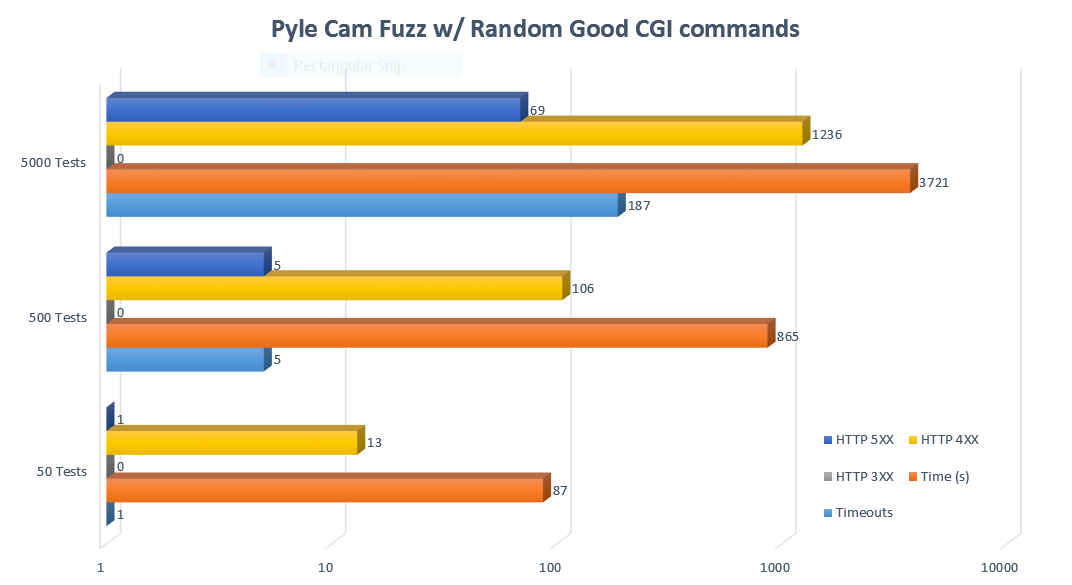
\includegraphics[width=0.9\linewidth]{Pyle_Good_CGI}
%\caption{ 5550 fuzz tests on Pyle camera with valid commands}
%\label{fig:Pyle_Good_CGI}
%\end{figure*}

%\begin{figure*}
%\centering
%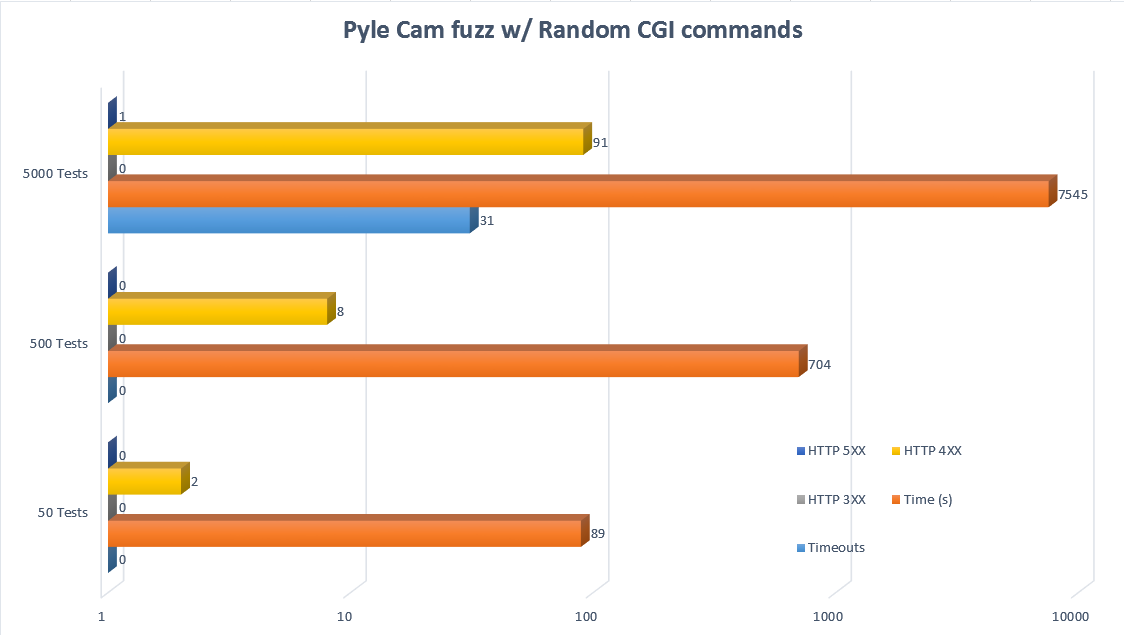
\includegraphics[width=0.9\linewidth]{Pyle_Rand_CGI}
%\caption{5550 fuzz tests on Pyle camera with random commands}
%\label{fig:Pyle_Rand_CGI}
%\end{figure*}



\subsection*{Acknowledgments}
We would like to thank our shepherd, Dr. Eric Eide in providing invaluable insight and assistance with two poor ECE students completing a CS project.

{\footnotesize \bibliographystyle{acm}
\bibliography{biblio}}




\end{document}






